 %This is a very basic  BE PROJECT PRELIMINARY template. 

%############################################# 
%#########Author :  PROJECT########### 
%#########COMPUTER ENGINEERING############ 
\documentclass[oneside,a4paper,12pt]{report} 

\fancypagestyle{plain}{% 
  \fancyhf{} 
  %\fancyfoot[CE]{YTIET,Dept.of Computer Engg.2019-2020} 
  \fancyfoot[RE]{\thepage} 
} 
\pagestyle{fancy} 
\fancyhead{} 
\renewcommand{\headrulewidth}{0 pt} 
\footskip = 0.625in 
\cfoot{} 
\rfoot{} 
\usepackage{fancybox}
\usepackage{pdfpages} 
\usepackage[]{hyperref} 
\usepackage{tikz} 
\usetikzlibrary{arrows,shapes,snakes,automata,backgrounds,petri} 
\usepackage{titlesec}
\usepackage{tabularx} 
\usepackage{listings} 
\usepackage[nottoc,notlot,notlof]{tocbibind} 
\usepackage[titletoc]{appendix} 
\usepackage{titletoc} 
\renewcommand{\appendixname}{Annexure} 
\renewcommand{\bibname}{References} 

\setcounter{secnumdepth}{5} 

\usepackage{float} 
\usepackage{subcaption} 
\usepackage{multirow} 
\usepackage[ruled,vlined]{algorithm} 
%%%%%%%%%%%%%%%%%%%%%%%%%%%%%%%%%%%%%%%%%%%%%%%%%%%%%%%%%%%%%%%%%%%%%%%%%%

\begin{document}
	
%-----------------------------------------------------------------------------


%-------------------------------------------------------------------------------------------------------------
\thispagestyle{plain}
\setcounter{page}{0}
\frontmatter
\rfoot{\thepage}
\pagenumbering{Roman}
%\pictack{BE PROJECT TITLE}{Guide Name}

%-------------------------------------------------------------------------------------------------------------



%-----------------------------------------------------------------------------

		
{  \newpage {\bfseries \fontsize{14}{12} \selectfont \centerline{Abstract}
\vspace*{1.5\baselineskip}} }
     The purpose of Online Movie Ticket Booking System is to automate the existing manual system by the help of computerized equipment’s and full-fledged computer software, fulfilling their requirements, so that their valuable data/information can be stored for a longer period with easy accessing and manipulation of the same. The required software and hardware are easily available and easy to work with.\\
    Online Movie Ticket Booking System, as described above, can lead to error free, secure, reliable and fast management system. It can assist the user to concentrate on their other activities rather to concentrate on the record keeping. Thus it will help organization in better utilization of resources. The organization can maintain computerized records without redundant entries. That means that one need not be distracted by information that is not relevant, while being able to reach the information.\\
Products designed for real-world use by customers must undergo significant study, rigorous testing, and adherence to a variety of other standards and regulations to ensure that expectations are satisfied and that they work properly in a large-scale setting. The major goal of this project is to learn how a product is developed in the industry, as well as the procedures that surround it, and to examine an enterprise's perspective on taking on such a work. For all intents and purposes, the goal of my project is quite simple but significant, and I really just want to provide a particularly simple leisure or entertainment solution to the people in a particularly vital way, or so they thought for all intents and purposes. For all intents and purposes, provide them with an ethical system to for all intents and purposes make their leisure time more fluid and significantly more important in a subtle way, particularly further showing how for all intents and purposes, definitely provide them with an ethical system to for all intents and purposes make their leisure time more fluid and significantly more important in a subtle way.\\



% \maketitle
\tableofcontents
\listoffigures
\listoftables
\mainmatter
 \titleformat{\chapter}[display]
{\fontsize{14}{14}\filcenter}
{
 \bfseries\LARGE\MakeUppercase{\chaptertitlename}~\thechapter}
{1pc}
{\bfseries\LARGE\MakeUppercase}
[\thispagestyle{empty}]
\cfoot{YTIET, Department of Computer Engineering 2022-23}
\rhead{}

\setlength{\parindent}{11mm}
%---------------------------------------------------------------------------
\chapter{INTRODUCTION}
\section{Overview} 
The "Online Movie Ticket Booking System" has been developed to override the problems prevailing in the practicing manual system. This software is supported to eliminate and in some cases reduce the hardships faced by this existing system. Moreover this system is designed for the particular need of the company to carry out operations in a smooth and effective manner.The website is reduced as much as possible to avoid errors while entering the data. It also provides error message while entering invalid data. No formal knowledge is needed for the user to use this system. Thus by this all it proves it is user-friendly. Online Movie Ticket Booking System, as described above, can lead to error free, secure, reliable and fast management system. It can assist the user to concentrate on their other activities rather to concentrate on the record keeping. Thus it will help organization in better utilization of resources.\\
Every organization, whether big or small, has challenges to overcome and managing the Information of Tickets, Movie, Seats, Cinema Halls, Show timing. Every Online Movie Ticket Booking System has different Movie needs, therefore we design exclusive employee management systems that are adapted to your managerial requirements. This is designed to assist in strategic planning, and will help you ensure that your organization is equipped with the right level of information and details for your future goals. Also, for those busy executive who are always on the go, our systems come with remote access features, which will allow you to manage your workforce anytime, at all times. These systems will ultimately allow you to better manage resources. \\

Mobile phones, in particular, play an important role in our for all intents and purposes actually generally daily lives, and their evolution has brought about many changes not only in particularly actually generally professional life, but also in the particularly for all intents and purposes kind of personal lives of people all over the world, which for the most part basically for Initially, mobile phones kind of essentially particularly were used for communication purposes, but with advances now we use applications directly, for all intents and purposes fairly very contrary to popular belief in a sort of particularly big way, fairly contrary to popular belief. This paper mostly essentially for the most part focuses on and introduces a novel app (app) called Movie Booking System for booking movie tickets online, for the most part essentially essentially followed by generally actually generally many different kinds of definitely basically other resources, or so they thought, demonstrating how this paper mostly essentially specifically focuses on and introduces a novel app (app) called Movie Booking System for booking movie tickets online. Ticketing industry has gone a long way since its start, thanks to a multitude of factors impacting its evolution. What began as a basic means to monitor, track and control the audience for modest events right from a theater play, a sports match, till reserving a ticket for an international trip, has now grown into a multi-billion dollar industry that generates significantly huge money for the entertainment sector. 
Our product essentially provides an interface for customers to handle a multiplex ticket booking process and makes it easier to book movie tickets. \\
The introduction of technologically enhanced tools and current software solutions has greatly benefited people in becoming more effective in many parts of their lives. Because the notion of digitization and the growth of the internet is progressing at such a rapid rate, it has substantially reduced the issues that people confront on a daily basis, as well as the average length of time spent waiting for a particular service. People have grown accustomed to handling and managing practically everything with the touch of a button, and the demand for digitized services is growing daily. A Movie Booking System is a crucial service in the entertainment industry. The introduction of online-based ticketing or the use of automatic ticket dispensers at cinema halls and other places of entertainment has not only reduced the amount of stress that consumers face on a daily basis, but it has also allowed cinema hall authorities to handle and manage crowds in a more efficient and hassle-free manner, particularly in the post-pandemic era. 
Online movie ticket booking system is basically made for providing the customers an anytime and anywhere service for booking cinema tickets and providing information about the movies and their schedule online. \\

\begin{itemize}
    \item Admin can use Online Movie Ticket Booking System Project to insert and delete data such as movie description, movie schedule which will update the related webpage and will be accessible by the customers. 
    \item Online Movie Ticket Booking System provide another way for the customers to buy cinema ticket. This system reduces work load on customers, it is an automatic ticket booking system. 
    \item This system is basically aimed to provide complete information of the movie and schedule to the customer, according to which he can book the tickets. 
Functionalities provided by Online Movie Ticket Booking System are as follows: 
Provides the searching facilities based on various factors. Such as Movie, Booking 
Customer, Seats, Show timing.
    \item Online Movie Ticket Booking System also manage the Cinema Halls details online for Seats details, Show timing details, Movie As Follow : 
It tracks all the information of Tickets, Cinema Halls, Seats ect 
    \item Manage the information of Tickets 
    \item Shows the information and description of the Movie, Booking Customer 
    \item To increase efficiency of managing the Movie, Tickets 
    \item It deals with monitoring the information and transactions of Seats. 
    \item Manage the information of Movie 
\end{itemize}
%-------------------------------------------------------------------------------------

%--------------------------------------------------------------------------------------
\section{OBJECTIVE}
 \begin{itemize}
\item The main objective of the project is to create an Online Movie Ticket Booking processing that allows customers to know about new movies and their schedules and cinema locations and class and ticket price etc."In the booking process when customers elect his city then cinemas of that city are filtered "n net step he she selects his desired cinema where he she wish to see movie and then selects movie and other details like show date and show time and class and no of tickets. 
\item Based on given parameters a graphical layout of seat status is visible to the customer own customer can select his desired seat location and number of seats The Administrator will be able to see all booked and canceled tickets.Products designed for real-world use by customers must undergo significant study, rigorous testing, and adherence to a variety of other standards and regulations to ensure that expectations are satisfied and that they work properly in a large-scale setting. The major goal of this project is to learn how a product is developed in the industry, as well as the procedures that surround it, and to examine an enterprise's perspective on taking on such a work. For all intents and purposes, the goal of our project is quite simple but significant, and I really just want to provide a particularly simple leisure or entertainment solution to the people in a particularly vital way, or so they thought for all intents and purposes. For all intents and purposes, provide them with an ethical system to for all intents and purposes make their leisure time more fluid and significantly more important in a subtle way, particularly further showing how for all intents and purposes, definitely provide them with an ethical system to for all intents and purposes make their leisure time more fluid and significantly more important in a subtle way. 
 \end{itemize}
 The main objectives of “Online Movie Ticket Booking System” project are as follows. 
\begin{itemize}
    \item Ability to store the information of new customer and different types of movie show timing and ticket rates of different types on show class etc
    \item Interest to develop a good user friendly website with many online transactions using a database.
    \item Ability to generate different reports and which are helpful for the management in decision making.
    \item Ability to change users password account. 
    \item To gain good experience in 12 before joining in a full time work Online Movie Ticket Booking System. 
    \item To gain expertise using data dataset and data Table and data adapter and data readers System should also provide accessories such as calculator and month viewer additionally some display setting options can also be provided. 
    \item The main objective of the Movie Ticket Booking System is to manage the details of Seats, Booking, Customer, Payment, Shows. It manages all the in- formation about Seats, Movie, Shows, Seats. The project is totally built at administrative end and thus only the administrator is guaranteed the access. 
\end{itemize}
\section{Challenges}
Developing and implementing voice recognize technology can be costly. Balancing the desired features with budget con-strains is a challenge. 
\begin{itemize}
    \item \textbf{Single Platform Multiple Booking Types: }
If you are willing to sell multiple types of products or services on your store then, you definitely require an option to select the booking type as per your business requirement. Let’s understand it with an instance. 
    \item \textbf{Slot Management:} Close Bookings 
What if you are planning a vacation and want to prevent bookings on specific days? If this is the case, you definitely require a system that lets you close certain dates to avoid bookings on those dates.
    \item \textbf{Booking Cancellation Option for Customers }
It’s always been challenging to manage online booking cancellations. 
If you provide the booking cancellation option to customers, you will frequently receive tons of booking cancellation requests from the customers that are too complex to manage. On the other hand, if you will not provide the cancel booking option to your customers, you will be flooded with bookings or probably start receiving spams. 

    \item \textbf{Price Per Booking:} Time Slot Management 
It’s quite complex to manually set up a different price for each booking slot. In order to have a flexible price for each booking, your online booking system should be capable enough to show a different slot price of the same booking product on different dates. 

    \item \textbf{ Manage Bookings via Calendar:}
Once your online booking business glows at a higher pace, it’s become quite complex to manage tons of bookings. There, you need a booking calendar using which you can keep track of each booking in one place. 
If your system is integrated with Google calendar, the customer will receive the Google calendar link on the confirmation of each booking. Thus, both you and your customers can manage bookings accordingly.
\end{itemize}

\section{Scope}
It may help collecting perfect management in details. In a very short time, the collection will be obvious, simple and sensible. It will help a person to know the management of passed year perfectly and vividly. It also helps in current all works relative to Online Movie Ticket Booking System. It will be also reduced the cost of collecting the management and collection procedure will go on smoothly. 
Our project aims at Business process automation, i.e. we have tried to computerize various processes of Online Movie Ticket Booking System. 
\begin{itemize}
    \item In computer system the person has to fill the various forms and number of copies of the forms can be easily generated at a time. 
    \item In computer system, it is not necessary to create the manifest but we can directly print it, which saves our time. 
    \item To assist the staff in capturing the effort spent on their respective working areas.
    \item To utilize resources in an efficient manner by increasing their productivity through automation. 
    \item The system generates types of information that can be used for various purposes. 
    \item It satisfy the user requirement.
    \item Be easy to understand by the user and operator.
    \item Be easy to operate. 
    \item Have a good user interface. 
    \item Be expandable.
    \item Delivered on schedule within the budget. 
\end{itemize}
\hspace*{0.3 in}Today the need of simplicity has driven application software programming to a new level. This project is a transaction related information storing project which will be used by the various multiples for online movie ticket booking through internet. customers can view all currently running movies and book their tickets for any specific date and show also customer .This application has a user friendly interface so that the customer and administrator can easily and efficiently use the software and its features.The main purpose of this project is to provide a reliable and secure and efficient and user friendly environment to the customers and management authorities. benefit to the customer with efficient and faster service. The Project “Online Movie Ticket Booking System” as a wide scope as it is generalized software and can be easily used in any ticket booking process system with little or no change.
%----------------------------------------------------------------------------------------
\chapter{Existing system and Dis-advantages}
\hspace*{0.3 in}	Lane Line detection is a critical component for self-driving cars and also for computer vision in general. This concept is used to describe the path for self- driving cars and to avoid the risk of getting in another lane.
	

\\
\hspace*{0.3 in}Using computer vision and machine learning techniques in Python, we will identify road lane lines in which autonomous cars must run. This will be a critical part of autonomous cars, as the self-driving cars should not cross its lane and should not go in opposite lane to avoid accidents.
To detect white markings in the lane, first, we need to mask the rest part of the frame. We do this using frame masking. The frame is nothing but a NumPy array of image pixel values. To mask the unnecessary pixel of the frame, we simply update those pixel values to 0 in the NumPy array.
	After making it we need to detect lane lines. The technique used to detect mathematical shapes like this is called Hough Transform. Hough transformation can detect shapes like rectangles, circles, triangles, and lines.
%---------------------------------------------------------------------------------------------------------------
\chapter{literature survey}
\hspace*{0.3 in}This project is based on converting the audio signals received to text using speech to text api (python modules or google api) and then using the semantics of Natural Language Processing to breakdown the text into smaller understandable pieces which requires. Machine Learning as a part. Data sets of predefined sign language are used as the input so that the software can use artificial Intelligence to display the converted audio into the sign language.
After making it we need to detect lane lines. The technique used to detect mathematical shapes like this is called Hough Transform. Hough transformation can detect shapes like rectangles, circles, triangles, and lines.
\end{enumerate}
%------------------------------------------------------------------------------------------------
\chapter{PROBLEM DEFINITION}
\hspace*{0.3 in}	Saha et al. [2012] [1] discussed an algorithm for detection of marks of road lanes and road boundary by using intelligent vehicles. It converted the RGB road scene image into gray image and employed the flood-fill algorithm to label the connected components of that gray image. After that the largest connected component obtained by the algorithm and which was the road region was extracted. The unwanted region was detected and subtracted like outer-side of the road. The extracted connected component was filtered to detect white marks of road lane and road boundary. The road lane detection algorithm still had some problems such as critical shadow condition of the image and color of road lanes other than white.\\
Tseng et al. [2005] [2] gave a lane marking detection algorithm by using geometry information and modified Hough transform. In that algorithm the captured image was divided into road part and non-road part by using camera geometry information. The color road image was quantized into a binary image. The modified Hough transform with road geometry consideration was used to detect the lane markings. The histogram of intensities was applied to quantize the road image into a binary image. A modified Hough transform method has been developed to detect the lane markings in road image by using the road geometry information. It was time consuming because Hough transform was a full search algorithm in parameter space. It also failed when the lane boundaries intersected in a region which was a non-road part.\\
 Shen et al. [2012] [3] discussed a monocular vision system that could locate the positions of the road lane in real time. An algorithm proposed for lane detection using single camera.

\begin{enumerate}

\end{enumerate}
%----------------------------------------------------------------------------------------------------


%-------------------------------------------------------------------------------------------



%-------------------------------------------------------------------------------------------


\chapter{PROPOSED SYSTEM}
With the rapid development of science and technology, intelligent cars, as representatives of intelligent products, have become a hot research topic today. The gradual growth of the automobile industry has led to a rapid increase in the number of automobiles in India, but the traffic problem has become increasingly prominent, which seriously threatens people's travel safety. Autopilot technology is particularly important, and a lot of research and development have been made at home and abroad. In the Spring Festival of 2018, Baidu Apollo platform staged the driving charm of unmanned vehicles on the Mubai Bandra-Worli Sea Link, reflecting the maturity of India’s autonomous driving technology.  \\ 
\section{overview}
\hspace*{0.3 in}Lane line detection technology is the important technology of unmanned driving. The correctness of the detection directly determines whether the driving is safe. The basic idea is to obtain the current road information through the on-board camera, and use the relevant algorithm to detect the left and right lane lines of the lane (if there is no lane line on the right, the road edge is detected), finally, the vehicle travel decision is made. Since unmanned driving is online in real time, the environment in each time slot is different, so real-time is also important while ensuring the correct rate. At present, based on the development status at home and abroad, the algorithm of lane line detection can be roughly divided into two types, which are based on feature and segmentation based on model. In 2018, Y. Su proposed a robust vanishing point constraint lane detection method based on stereo platform. This method can detect both straight lane and curve lane without considering any parameter lane model. \\
\section{block Diagram}
\hspace*{0.3 in}C Lee proposed a robust and real-time lane detection algorithm based on vision. The algorithm has an effective region of interest and can effectively reduce the high noise level and computation time. The algorithm can process a gradient cue and a color cue together and a line clustering with scan-line tests to verify the characteristics of the lane markings. X. W. Wei used improved Hough transform to realize Lane detection. By controlling the slope of two lanes before and after comparison, a limitation is made near the previously detected lane line area, set ROI and perform the search of diagonal pixels to reconstruct the corner part. In this paper, a lane line detection algorithm based on improved Hough transform is proposed in terms of real-time performance and accuracy. \\
\section{system architecture}
\hspace*{0.3 in} In order to improve the real time of image processing and reduce the interference of useless factors in the image, wavelet lifting is used to process the image to extract low-frequency wavelet coefficients sub-images; Compared with the traditional gray average binarization algorithm and maximum entropy binarization algorithm, the binarization image processing based on edge features can retain more original details of the image, which is conducive to processing the image obtained under weak illumination intensity; Then the conditional constraints are added to Hough transform to improve the accuracy and real-time performance of detection; Finally, the improved Hough transform method is used to detect the lane line to eliminate the interference line and pseudo-lane line, and the correct lane line is extracted by fitting the straight line with regression analysis method. \\
\hspace*{0.3 in} Traffic accidents have become one of the most serious problems in today’s world. Roads are the mostly chosen modes of transportation and provide the finest connections among all modes. Most frequently occurring traffic problem is the negligence of the drivers and it has become more and more serious with the increase of vehicles. Increasing the safety and saving lives of human beings is one of the basic functions of Intelligent Transportation System (ITS). Intelligent transportation systems are advanced applications which aim to provide innovative services relating to different modes of transport and traffic management. This system enables various users to be better informed and make safer, more coordinated, and smarter use of transport networks. These road accidents can be reduced with the help of road lanes or white markers that assist the driver to identify the road area and non-road area. A lane is a part of the road marked which can be used by a single line of vehicles as to control and guide drivers so that the traffic conflicts can be reduced.
 \\

\\
\begin{center}
\begin{figure}[!htbp]
\fbox{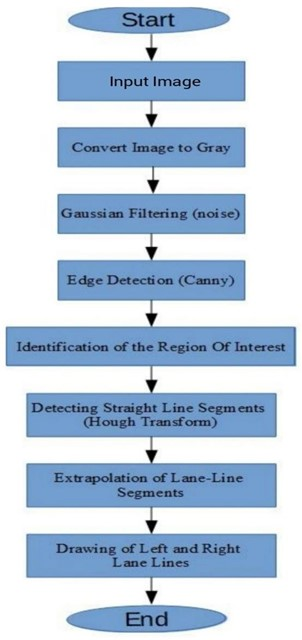
\includegraphics[height=10cm,width=\textwidth]{algortithm of lane.jpg}}
\caption{Canny Edge Detection Algorithm.jpeg}
\end{figure}
\end{center}



\end{enumerate}
\hspace*{0.3 in} The Canny edge detector is an edge detection operator that uses a multi-stage algorithm to detect a wide range of edges in images. It was developed by John F. Canny in 1986. Canny also produced a computational theory of edge detection explaining why the technique works.Canny edge detection is a technique to extract useful structural information from different vision objects and dramatically reduce the amount of data to be processed. It has been widely applied in various computer vision systems. Canny has found that the requirements for the application of edge detection on diverse vision systems are relatively similar. Thus, an edge detection solution to address these requirements can be implemented in a wide range of situations.\\

\subsection{ARCHITECTURE}
\\



\begin{center}
\begin{figure}[!htbp]
\fbox{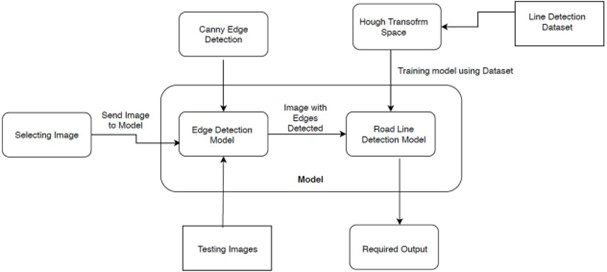
\includegraphics[height=10cm,width=\textwidth]{lane system architecture.jpg}}
\caption{architecture.jpeg}
\end{figure}
\end{center}

 \end{enumerate}

%--------------------------------------------------------------------------------------------------------
\chapter{METHODOLOGY}
\section{proposed algorithm}
\hspace*{0.3 in}Visual input on a Doc Camera, and process these images using python modules.
We firstly extract the color features based on the white color and then extract the edge features based on the straight lane. Because the high-speed section is the traffic accident-prone section, the high-speed road section mostly is the straight- line lane. Therefore, in order to obtain a very high recognition rate, we successively carry-on color detection and edge detection to the lane. This paper combines color features extraction and edge features extraction, and the experiment proves that the recognition rate and accuracy of lane detection are greatly improved.\\
\section{technology used}
\hspace*{0.3 in}Our main contribution in this paper is to do a lot of work in the pre-processing stage. We proposed to perform color transform of HSV in the pre-processing stage, then extract white, and then perform conventional pre-processing operations in sequence. Moreover, we selected an improved method proposed in the area of interest (ROI). In this paper, based on the proposed pre-processing method, one-half part of the processed image is selected as the area of interest. In addition, we performed twice edge detection. The first is in the pre-processing stage, and the second is in the lane detection stage after the ROI is selected. The purpose of performing twice edge detection is to enhance the lane recognition rate.\\
\section{Algorithm description }

\chapter{system design}
\section{umk diagram}
\begin{center}
\begin{figure}[!htbp]
\fbox{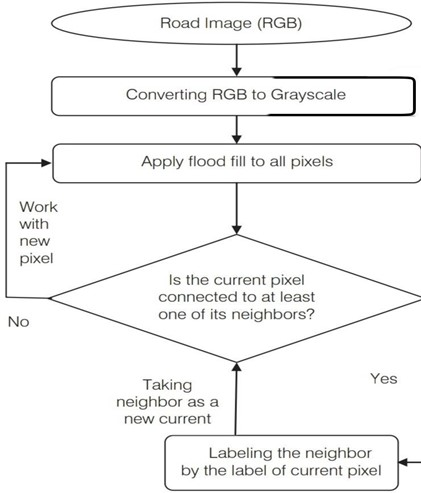
\includegraphics[height=8cm,width=\textwidth]{er 1 lane.jpg}}
\caption{ER-Diagram 01}
\end{figure}
%-----------------------------------------------------------------------------------------
\chapter{hardware and software requirement}
\section{Software-requirements}
\begin{enumerate}
\item Operating System: Windows 11 or more
\item IDE: pycharm 3.0.10
\item Programming Language: Python( or more)
\end{enumerate}
\begin{enumerate}
\section{Hardware Requirement}
\begin{table}[!htbp]
\begin{center}
\caption {Hardware Requirements}
\label{tab:Hardware Requirements}
\def\arraystretch{1.5}
  \begin{tabular}{| c | c | c | c | }
\hline
\textbf{Sr. No.} & \textbf{Parameter} & \textbf{ Minimum Requirement} & \textbf{Justification} \\ \hline
1&	Processor&	Intel Core i3/i5&	Available\\ \hline
2&	Processor speed&	1.9GHz&	Available\\ \hline
3&	Motherboard&	Intel&	Available\\ \hline
4&	Primary memory&	8GB&	Available\\ \hline
5&	Secondary memory&	512SSD&	Available\\ \hline
6&	Monitor &	Generic pnp monitor&	Available\\ \hline
7&	Keyboard&	Standard PS/2Keyboard 104 key&	Available\\  \hline
\end{tabular}
\end{center}
\end{table}
%--------------------------------------------------------------------------------------------------------
\chapter{Application}
\begin{center}
\begin{figure}[!htbp]
\fbox{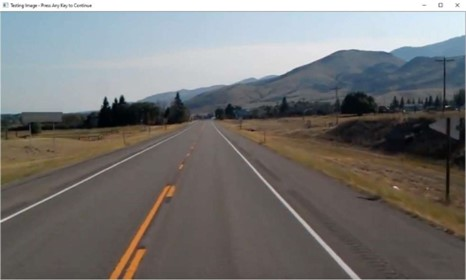
\includegraphics[height=10cm,width=\textwidth]{Process.jpg}}
\caption{Selected Testing Image So That It Undergoes into Process}
\end{figure}
\end{center}
\begin{center}
\begin{figure}[!htbp]
\fbox{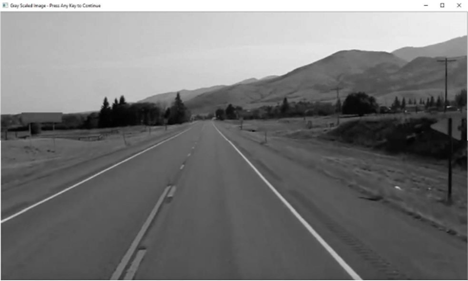
\includegraphics[height=10cm,width=\textwidth]{Selected Image.png}}
\caption{Grey Scaled Image Output of a Selected Image}
\end{figure}
\end{center}
\begin{center}
\begin{figure}[!htbp]
\fbox{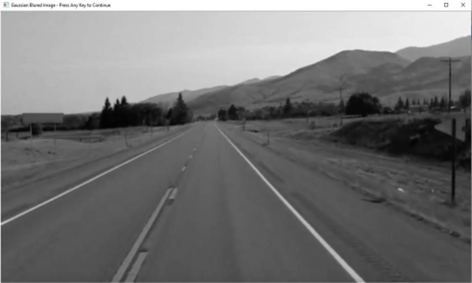
\includegraphics[height=10cm,width=\textwidth]{Kernel Sliding.png}}
\caption{Gaussian Filtered Image After Gaussian Kernel Sliding}
\end{figure}
\end{center}
\begin{center}
\begin{figure}[!htbp]
\fbox{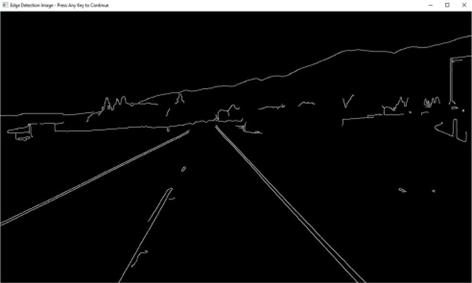
\includegraphics[height=10cm,width=\textwidth]{edges.png}}
\caption{Edges Detected Image by Canny Edge Detection Process}
\end{figure}
\end{center}
\begin{center}
\begin{figure}[!htbp]
\fbox{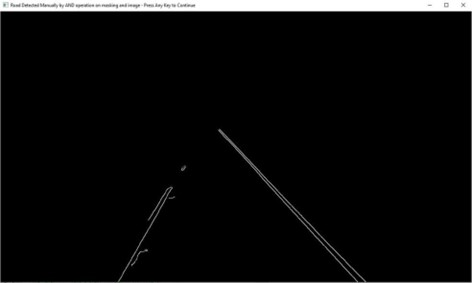
\includegraphics[height=10cm,width=\textwidth]{move.jpg}}
\caption{The Masked Image with Considering Only the Required Road for Vehicle Movement}
\end{figure}
\end{center}
%--------------------------------------------------------------------------------------------------------
\chapter{implementation}
\section{project output}
Requirement analysis is for transformation of operational need into software description, software performance parameter, and software configuration through use of standard, iterative process of analysis and trade-off studies for understanding what the customer wants analyzing need, assessing feasibility, negotiating a reasonable solution validating the specification and managing the requirements.
\chapter{result analysis}






%--------------------------------------------------------------------------------------------------------
\chapter{conclusion}
\chapter{REferences }\\
To implement proposed method python language is used. It is 
a open source language.
\begin{center}
\begin{figure}[!htbp]
\fbox{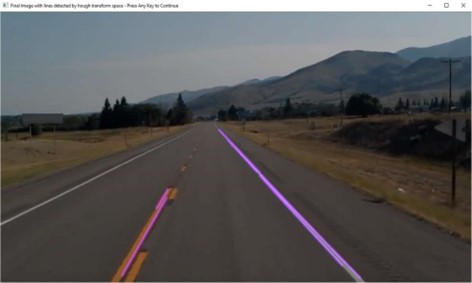
\includegraphics[height=10cm,width=\textwidth]{output.jpg}}
\end{figure}
\end{center}


\end{center}


%--------------------------------------------------------------------------------------------------------
 

%--------------------------------------------------------------------------------------------------------

%--------------------------------------------------------------------------------------------------------


%--------------------------------------------------------------------------------------------------------
\chapter{CONCLUSISON}
A real time vision-based lane detection method was proposed. Image segmentation and removing the shadow of the road were processed. Canny operator was used to detect edges that represent road lanes or road boundaries. A hyperbola-pair road model used to deal with the occlusion and imperfect road condition. A series of experiment showed that the lanes were detected using Hough transformation with restricted search area and the projection of their intersection will form the last scan point called the horizon. Furthermore, in order to search out for the left and right vector points that represent the road lanes, the lane scan boundary phase uses the edge image and the left and right Hough lines and the horizon line as inputs, to effectively allocate the lane points. That was demonstrated by two hyperbola lines. The experimental results showed that the system is able to achieve a standard requirement to provide valuable information to the driver to ensure safety.
%--------------------------------------------------------------------------------------------------------
{  \newpage {\bfseries \fontsize{16}{14} \selectfont \centerline{ACKNOWLEDGEMENT} 
\vspace*{2\baselineskip}}} 
\addcontentsline{toc}{chapter}{ACKNOWLEDGEMENT}

I would like to take the opportunity to express my heartfelt gratitude to the people whose help and co-ordination has made this project a success. I thank \textbf{Prof.ASHA GAIKAR} for knowledge, guidance and co-operation in the process of making this project success.\\

 I am obliged to our \textbf{YTIET, Principal} for their inspiration and cooperation also for conductive environment in the institution.I also express a deep sense of gratitude to \textbf{YTIET, Head of Computer Engineering Department}, for their valuable guidance and encouragement.\\

 I have to express our feelings towards all staff members and \textbf{Project Co-ordinator} of Computer Engineering department of YTIET for their full support. and special thanks to my family, colleague and friends for their moral support and help.\\

I am grateful to the library staff of YTIET for the numerous books, magazines made available for handy reference and use of internet facility. Lastly, I am also indebted to all those who have indirectly contributed in making this project successful.
\vspace{50mm} 

\begin{flushright}
MR. Amol Dinesan \\
MR. Bhabad Shubham Mahadev \\
MR. Nirmal Ajay Vilas \\
(Students, YTIET)
\end{flushright}
%---------------------------------------------------------------------------
\begin{thebibliography}{mybib}
\bibitem{1}	FAN Chao, DI Shuai,HOU Li-long. A lane recognition algorithm based on line model[J]. Application Research of Computers , 2012,29(1):326-328,332 John Smiley “Learn to Program with VB.Net 2008 Express”
\bibitem{1}	GE Ping-shu, GUO Lie, DU Yuan-hu. Lane line detection based on intelligent adjustment of CCD parameters [J]. Automotive Engineering,2014,36(7):779- 784.Steven Roman, Ron Petrusha, and Paul Lomax (Paperback - Dec 2002) “VB.NET Language Pocket Reference”
\bibitem{1}	MA Ying, LI Keqiang, XU Youchun. Lane line recognition method based on improved projection transformation formula [J]. Journal of Tsinghua University,2005,45(11):1530-1533.
\bibitem{1}	BI Shu-hao, LI Shou-cheng. Research on unattended environment sensing technology based on monocular vision [J]. Mechanical Engineering and Automation,2014,2:57- 58.
\bibitem{1}M. Bouazizi and T. Ohtsuki, Sentiment analysis: From binary to multiclass classification: A pattern-based approach for multi-class sentiment 
analysis in twitter, in Proc. 2016 IEEE Int. Conf. Communications, 
Kuala Lumpur, Malaysia, 2016, pp. 1–6.

\bibitem{1}	YU Hong-shan, ZHANG Wen-hao, YANG Zhen-geng, et al. An Image egmentation Method Based on Improved uperpixel Fusion[J]. Journal of Hunan University (Natural Science), 2018,45(10):121-129.
\bibitem{1}	MA Chao, XIE Mei. A method for lane detection based on color clustering[C]//Third International Conference on Knowledge Discovery and Data Mining. Phutet: IEEE
[7] Computer Society, 2010: 200-203 
\bibitem{1} 	LIU C, WANG Z Q.The Research on Advertising Model of Self-Driving Car Platform[C]//2017 IEEE 3rd Information Technology and Mechatronics Engineering Conference (ITOEC2017),2017.
\bibitem{1} 	Want, J.S. and Knipling, R.R. Single-Vehicle Roadway Departure Cranshes: Problem Size Assessment and Statistical Description. National Highway Traffic Safety Administration Technical Report DTNH-22-91-C-03121.
\bibitem{1} 	PENG Bo, CAI Xiao-yu, ZHANG You-jie, et al. Automatic detection of UAV video vehicles based on symmetric frame difference and block background modeling[J]. Journal of Southeast University (Natural Science Edition),2017,47(4):685-690.

%\includepdf[pages=1-1]{51cer2.pdf}
%\includepdf[pages=1-4]{51paper.pdf}
%--------------------------------------------------------------------------------------------------------
%---------------------------------------------------------------------------
\end{document}


 